\chapter{Funzione \emph{floor} e \emph{ceil}}
\paragraph{floor} La funzione \emph{floor}(x) restituisce il più grande intero minore o uguale ad $x$
$$\mathrm{floor}(x)=\lfloor
x\rfloor\stackrel{\mathit{def}}{=}\max\{n\in\mathbb{Z} | n\leq
x\}$$
\paragraph{ceil} La funzione \emph{ceil}(x) restituisce il più piccolo intero maggiore o uguale a $x$
$$\mathrm{ceil}(x)=\mathrm{ceiling}(x)=\lceil
x\rceil\stackrel{def}{=}\min\{n\in\mathbb{Z} | n\geq x\}$$
\paragraph{Esempi a confronto}
\begin{align*}
	\text{\textbf{\textit{floor}}}&&\text{\textbf{\textit{ceil}}}&\\
	\lfloor 3 \rfloor &=3&\lceil 3 \rceil &=3\\
	\lfloor 2.6 \rfloor &=2&\lceil 2.6 \rceil&=3\\
	\lfloor -2.6 \rfloor &=-2&\lceil -2.6 \rceil&=-3
\end{align*} 
\begin{center}
	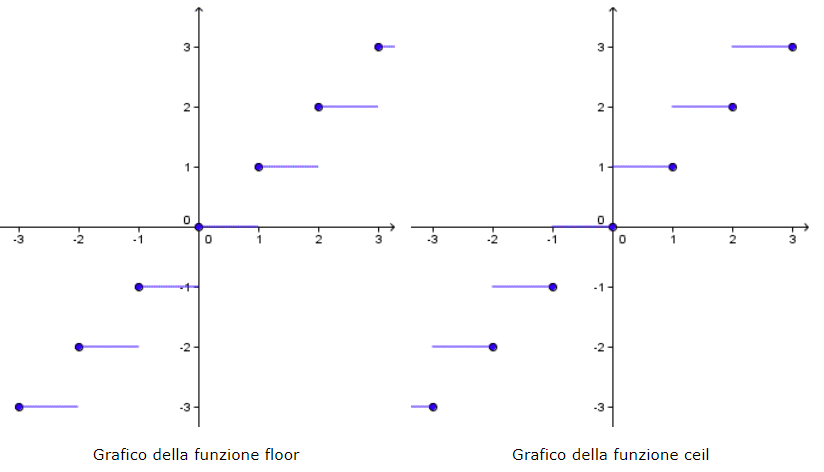
\includegraphics[scale=.7]{19.PNG}
\end{center}
\[\boxed{\text{\url{http://www.batmath.it/interattive/ggb_tutorials/floor_ceil/floor_ceil.htm}}}\]
\chapter{Operatore XOR}
Molto spesso la professoressa utilizza come sinonimo di XOR la frase \emph{somma in modulo 2}. La cosa torna se andiamo a rivedere alcune cose viste a Reti logiche. 

\section*{\emph{Full adder} in base 2}
A Reti logiche abbiamo visto le caratteristiche dell'addizione nell'insieme dei numeri naturali. In particolare, abbiamo fatto la sintesi del \emph{full adder} in base 2, cioè un sommatore a una cifra. Al di la del \emph{carry} $C_{out}$ dobbiamo ricordarci come viene ottenuto $S_i$.
\begin{center}
	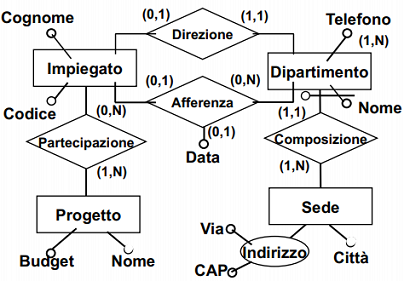
\includegraphics[scale=.59]{20.PNG}
\end{center}
$S_i$ è ottenuto a partire da una porta XOR a tre ingressi (dove si considera anche $C_{in}$).

\section*{Elemento neutro ed elemento non neutro dello XOR}
\small 
\begin{itemize}
	\item \textbf{Zero elemento neutro}: $x \oplus 0 = x$, cioè $1 \oplus 0 = 1, 0 \oplus 0=0$
	\item \textbf{Uno elemento non neutro}: $x\oplus 1 = \overline{x}$, cioè $0 \oplus 1 =1, 1 \oplus 1 = 0$
\end{itemize} 
\normalsize 